\newpage
\section{Auswertung}
\label{sec:Auswertung}

\subsection{Heizrate}
\label{sec:heiss}
Zunächst ist es sinnvoll die Heizrate bei dem Versuch zu untersuchen, da diese händisch immer wieder nachgeregelt und dardurch verändert wurde. Dazu bietet sich an 
die gemessene Temperatur gegen die Zeit aufzutragen und eine lineare Regression durchzuführen.

Die gefittete Funktion hat die Form
\begin{equation*}
  T(t) = b \cdot t + T_0 \, .
\end{equation*}

\noindent
Aus dieser, dass für die Messung in 1,5er Temperaturschritten eine Heizrate $b_1$ und bei 2er Temperaturschritten eine Heizrate von $b_2$ vorliegt. 
\begin{align*}
  &b_1 = \SI{1.41(13)}{\kelvin\per\minute} \\
  &b_2 = \SI{1.93(33)}{\kelvin\per\minute} \, .
\end{align*}

Die Notation die Variablen die sich auf die Messung mit 1,5er Temperaturschritten bezieht mit $_1$ und die Variablen welche sich auf die Messung mit 2er Temperaturerhöhungsschritten 
bezieht mit $_2$ zu vermerken wird in dem gesamten \autoref{sec:Auswertung} und \autoref{sec:Diskussion} beibehalten.

\noindent
Die \autoref{fig:2-linregress} sind mit den entsprechenden gefitteten Funktion aufgetragen.

\begin{figure}
  
  \centering
  \begin{subfigure}[b]{0.45\textwidth}
      \centering
      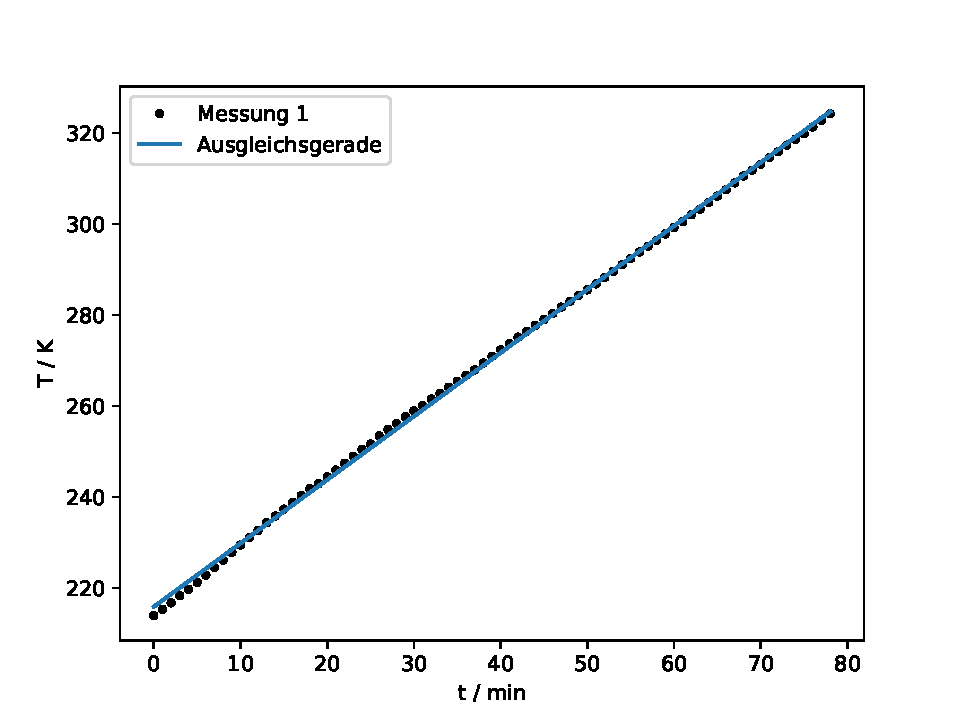
\includegraphics[width=\textwidth]{build_j/zeit_temp_fit_1.pdf}
      \caption{Die gemessene Temperatur gegen die Zeit aufgetragen für die Messung 1 inklusive Fit Funktion}
  \end{subfigure}
  \hfill
  \begin{subfigure}[b]{0.45\textwidth}
      \centering
      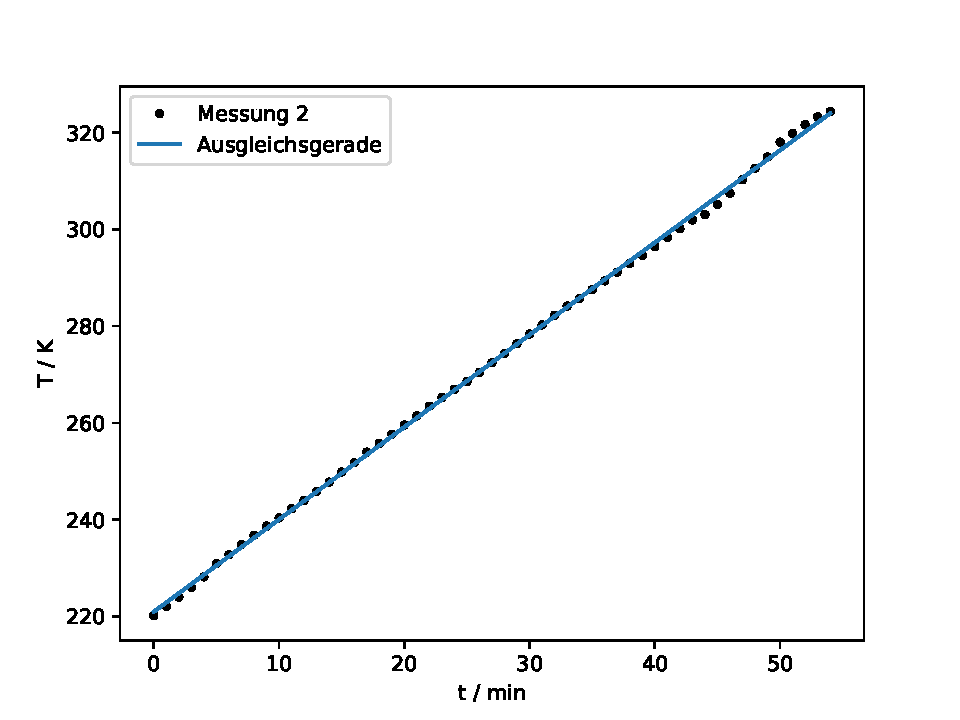
\includegraphics[width=\textwidth]{build_j/zeit_temp_fit_2.pdf}
      \caption{Die gemessene Temperatur gegen die Zeit aufgetragen für die Messung 2 inklusive Fit Funktion}
  \end{subfigure}
  \caption{}
  \label{fig:2-linregress}
\end{figure}


\subsection{Untergrund}

Da bei der Messung der Daten nicht nur der Strom der durch die Dipolrelaxationen im Kristall gemessen wurde, sondern auch ein exponentiell wachsender Untergrund, ist es sinnvoll
für die weitere Auswertung diese durch eine e-Funktion der Form 
\begin{equation*}
  f(T) = a \cdot \exp(-\frac{m}{T})
\end{equation*}

\noindent 
zu approximieren. Das Temperatur-Strom Diagramm inklusive der gefitteten e-Funktion ist in \autoref{fig:Untergrund} zu sehen. Der Fit wird versucht an das 2. Maxima zu legen. 
Daraus folgen folgende Werte:

\begin{align*}
  &a_1 =  \SI{6.197(3794)e11}{\pico\ampere} &&  m_1 = \SI{7282.75(18414)}{\kelvin} \, ,\\
  &a_2 = \SI{1.263(617)e11}{\pico\ampere} &&  m_2 = \SI{6729.57(15056)}{\kelvin} \, .\\ 
\end{align*}


\begin{figure}
  
  \centering
  \begin{subfigure}[b]{0.75\textwidth}
      \centering
      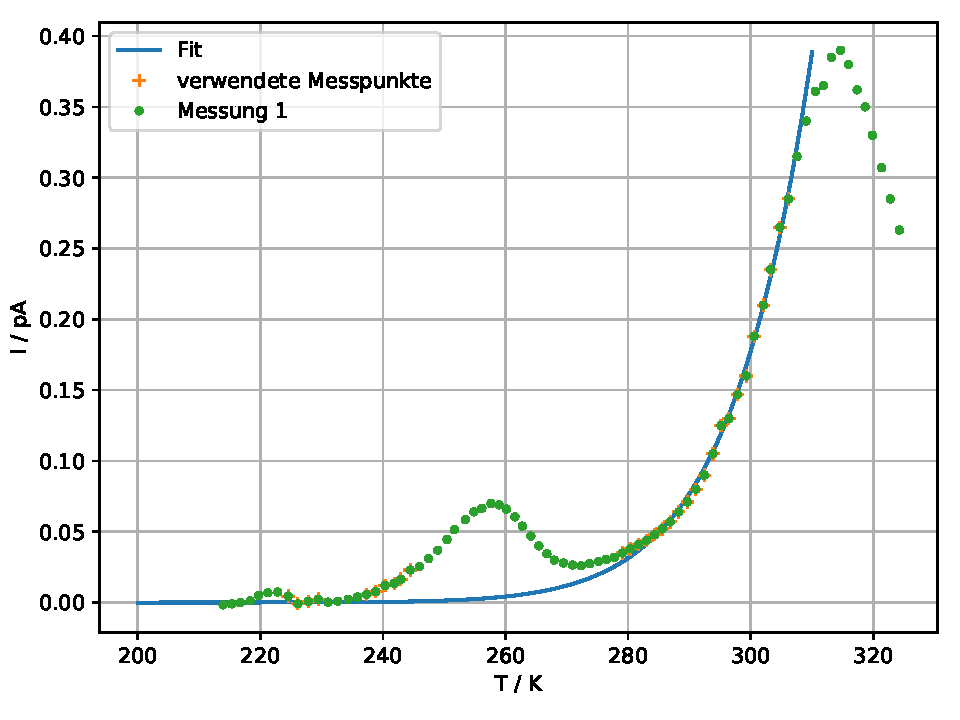
\includegraphics[width=\textwidth]{build_j/untergrund_1.pdf}
      \caption{Die gemessene Temperatur gegen den gemessenen Strom aufgetragen für die Messung 1 inklusive Fit für den Untergrund}
  \end{subfigure}
  \hfill
  \begin{subfigure}[b]{0.75\textwidth}
      \centering
      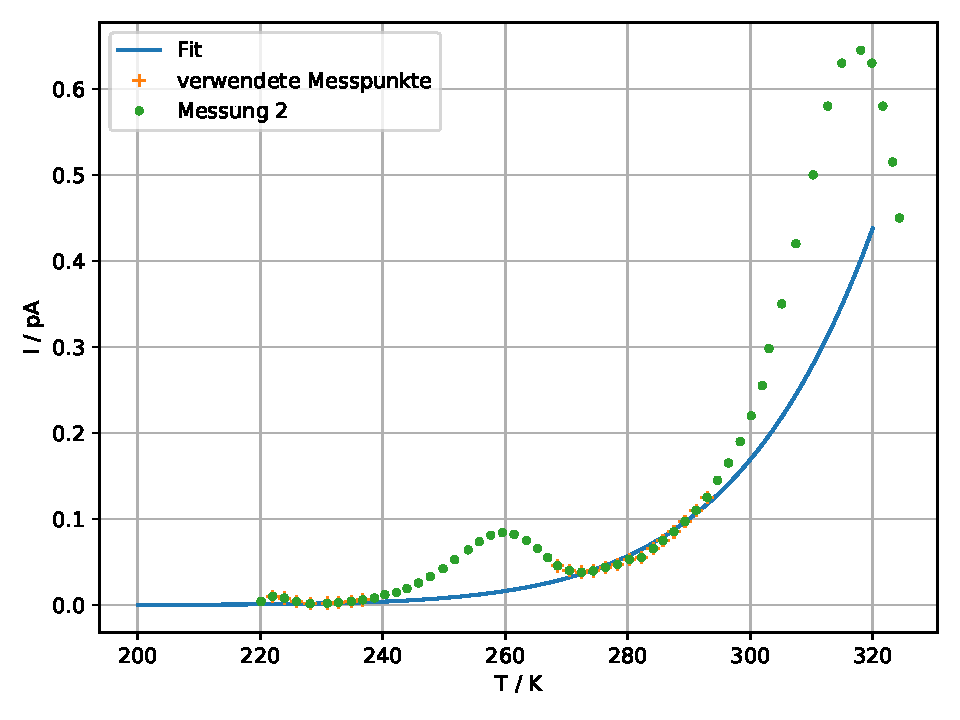
\includegraphics[width=\textwidth]{build_j/untergrund_2.pdf}
      \caption{Die gemessene Temperatur gegen den gemessenen Strom aufgetragen für die Messung 1 inklusive Fit für den Untergrund}
  \end{subfigure}
  \caption{}
  \label{fig:Untergrund}
\end{figure}

\subsection{Berechnung der Aktivierungsenergie über den Strom}
Es gibt 2 Möglichkeiten den Aktivierungsenergie zu bestimmen. Die erste Möglichkeit ergibt sich aus dem Zusammenhang (\ref{eqn:approx}). Dabei aknn von diesem der natürliche
Logarithmus gebildet werden und die Stromdichte in den Strom mithilfe der Querschnittsfläche durchwelche er fließt überführt werden. So ergibt sich 
\begin{equation}
    \ln\left(I(T)\right) = \underbrace{\ln\left(A \frac{p^2E}{3 k_\text{B} T} \frac{N_p}{\tau_0}\right)}_{\text{const.}} - \underbrace{\frac{W}{k_\text{B}}}_{\text{Steigung}} \frac{1}{T} \, .
    \label{eqn:geradengleichung}
\end{equation}
und damit folgt für die Aktivierungs $W$ der Zusammenhang
\begin{equation}
    W = m \cdot k_\text{B} \, ,
    \label{eqn:Aktivierungsenergie}
\end{equation}
wobei $m$ die Steigung dargestellt.

\noindent
Durch diese Form bietet sich, zur Bestimmung der Energie, ein Fit der Form 
\begin{equation*}
  \ln{I(T)} = c - m \cdot \frac{1}{T} \, .
\end{equation*}

\noindent
an. Die Fits sind in \autoref{fig:met1} dargestellt. Aus diesen folgen die Werte
\begin{align*}
  c_1 =  \SI{32.61(201)}{\ln(\pico\ampere)}& && m_1 = (-8970.35\pm 493.21)\,\si{\kelvin} \,  \\
  c_2 =  \SI{28.24(180)}{\ln(\pico\ampere)}& && m_2 = (-7903.24\pm 448.18)\,\si{\kelvin} \, , \\
\end{align*}

\noindent
womit sich die Aktivierungsenergie $W$ bestimmen lässt zu 

\begin{align*}
  & W_{1} = \SI{1.24(7)e-19}{\joule} = \SI{0.77(4)}{\electronvolt} \,  \\
  & W_{2} = \SI{1.09(6)e-19}{\joule} = \SI{0.68(4)}{\electronvolt} \, . \\
\end{align*}


\begin{figure}
  
  \centering
  \begin{subfigure}[b]{0.75\textwidth}
      \centering
      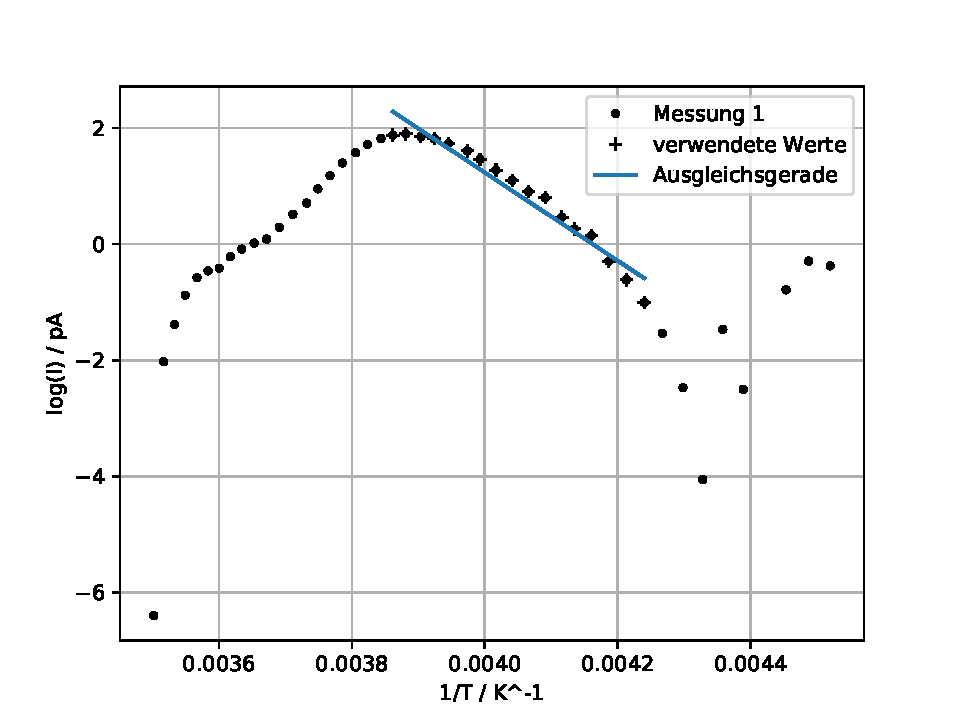
\includegraphics[width=\textwidth]{build_j/log(I)_1durchT_1.pdf}
      \caption{Inverse Temperatur gegen den logarithmus des gemessenen Strom aufgetragen für die Messung 1 inklusive Ausgleichsgeraden für die Bestimmung der Energie.}
  \end{subfigure}
  \hfill
  \begin{subfigure}[b]{0.75\textwidth}
      \centering
      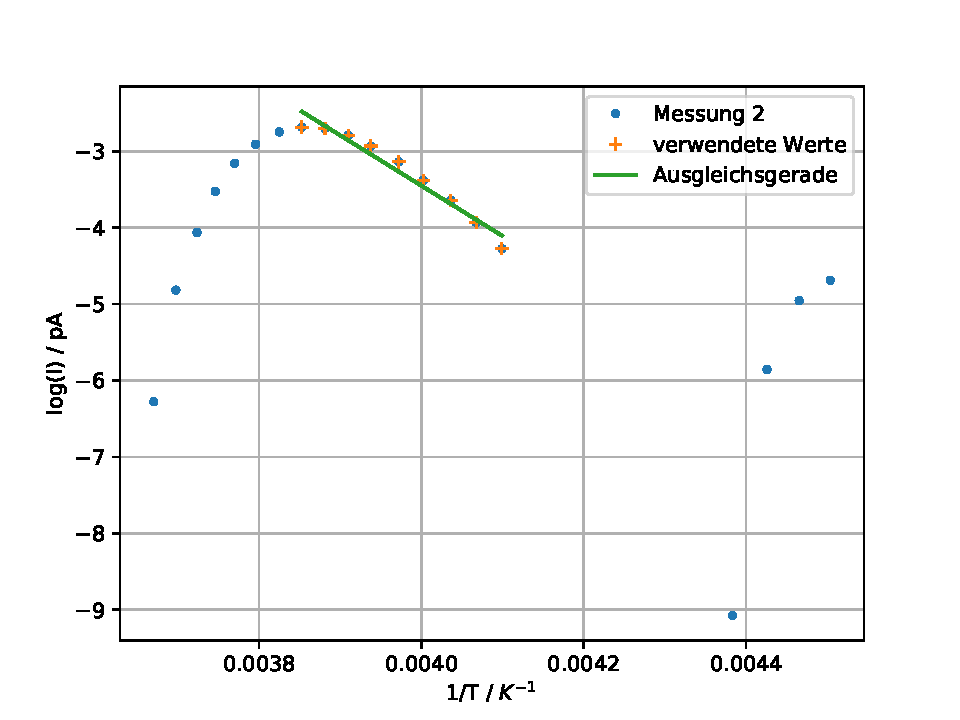
\includegraphics[width=\textwidth]{build_j/log(I)_1durchT_2.pdf}
      \caption{Inverse Temperatur gegen den logarithmus des gemessenen Strom aufgetragen für die Messung 2 inklusive Ausgleichsgeraden für die Bestimmung der Energie.}
  \end{subfigure}
  \caption{}
  \label{fig:met1}
\end{figure}


\subsection{Bestimmung der Aktivierungsenergie nach der Integrationsmethode}

Die 2. Methode der Bestimmung der Aktivierungsenergie lässt sich über die \autoref{eqn:idkwhat} bewerkstelligen. Dazu wird, wie zuvor, $\frac{1}{T}$ aufgetragen, diesmal jedoch gegen
das Integral $\ln\left( \frac{\int_T^\infty I(T') \, \text{d}T'}{b \tau_0 \cdot I(T)}\right)$. Dieses wird nummerisch bestimmt und mithilfe des Pieks und einer linearen Regression 
der Form 
\begin{equation*}
  y = a \cdot x + b \, .
\end{equation*}

\noindent
Diese liefert die Werte 

\begin{align*}
  &a_1 = (9541,25 \pm 135,01)\,\si{\kelvin}  && b_1 = -34,97 \pm  \, 0,54 , \\ 
  &a_2 = (8502.93 \pm 366.29)\,\si{\kelvin} && b_2 = -30,63 \pm 1,42\, . \\ 
\end{align*}

\noindent
somit kann die Aktivierungsenergie $W$ nach der \autoref{eqn:idkwhat} bestimmt werden

\begin{align*}
  W_{1} &= \SI{1.37(4)e-19}{\joule} &= \SI{0.858(024)}{\electronvolt} \, \\
  W_{2} &= \SI{1.17(5)e-19}{\joule} &= \SI{0.733(032)}{\electronvolt} \, .\\
\end{align*}

\noindent
Die Grafiken zur Visualisierung sind in \autoref{fig:int} zu finden.

\begin{figure}
  
  \centering
  \begin{subfigure}[b]{0.75\textwidth}
      \centering
      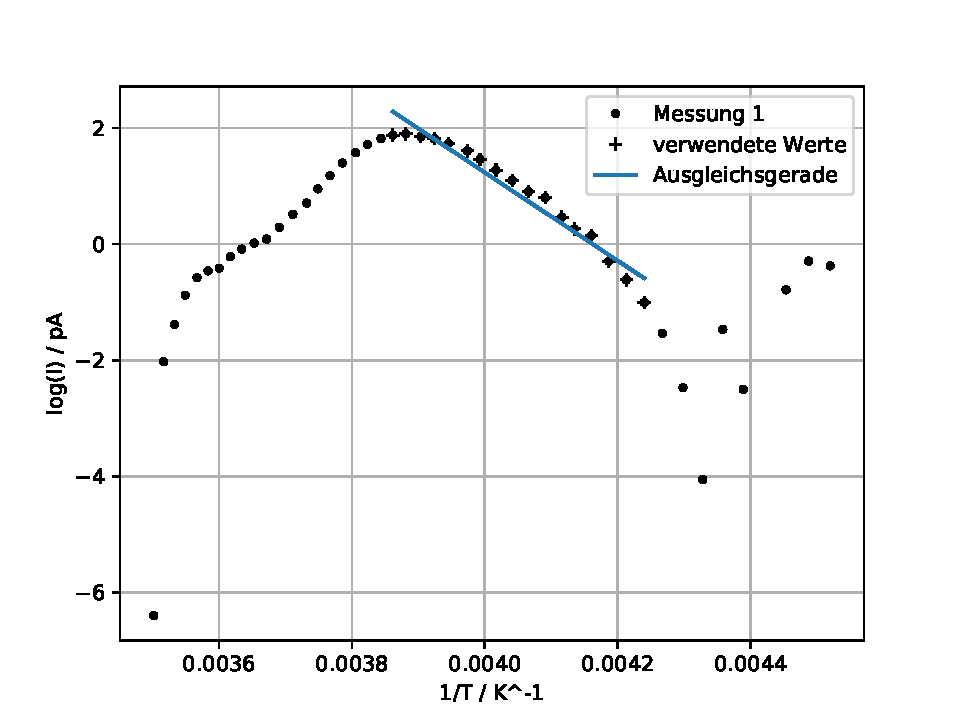
\includegraphics[width=\textwidth]{build_j/log(I)_1durchT_1.pdf}
      \caption{Inverse Temperatur gegen den logarithmus des gemessenen Strom aufgetragen für die Messung 1 inklusive Ausgleichsgeraden für die Bestimmung der Energie.}
  \end{subfigure}
  \hfill
  \begin{subfigure}[b]{0.75\textwidth}
      \centering
      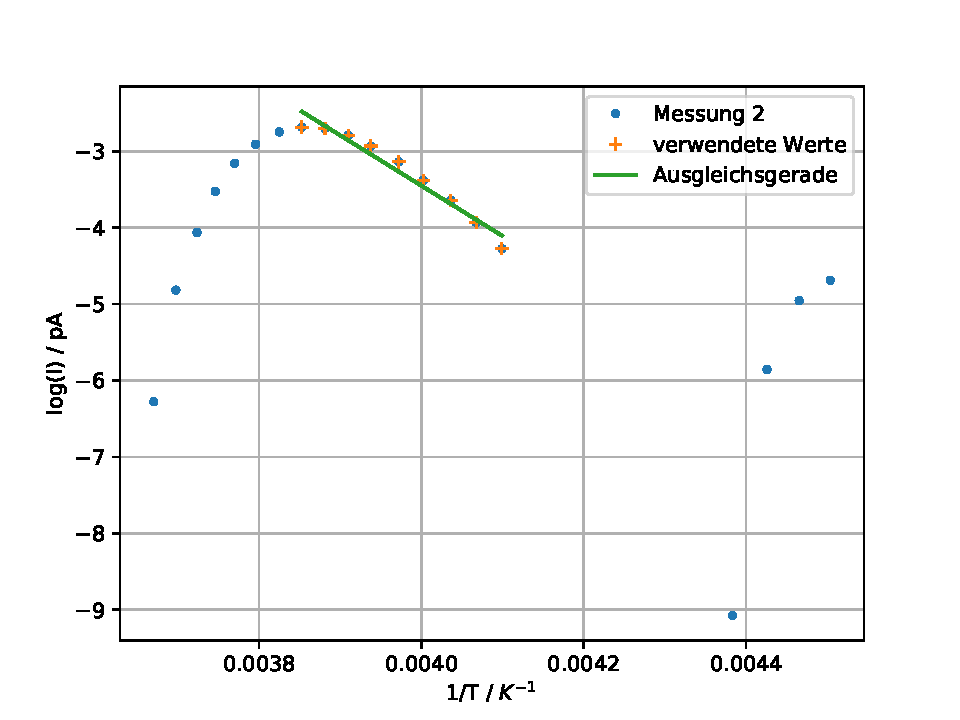
\includegraphics[width=\textwidth]{build_j/log(I)_1durchT_2.pdf}
      \caption{Inverse Temperatur gegen den logarithmus des gemessenen Strom aufgetragen für die Messung 2 inklusive Ausgleichsgeraden für die Bestimmung der Energie.}
  \end{subfigure}
  \caption{}
  \label{fig:int}
\end{figure}

\subsection{Relaxationszeit}
Zusätzlich zu der Aktivierungsenergie kann die Relaxationszeit berechnet werden (\ref{eqn:tau}). Dazu werden die Heizraten aus \autoref{sec:heiss} genutzt, sowie die 
bereits berechneten Aktivierungsenergien.

\noindent
Die Relaxationszeit für die erste Methode lautet 

\begin{align*}
  \tau_{1} =  (3 \pm 5)\cdot 10^{-15}\,\si{\minute} &&  \tau_{2} = (5 \pm 8)\cdot 10^{-15}\,\si{\minute}\,  \\ 
\end{align*}

und für die zweite Methode

\begin{align*}
  \tau_{1} =  ( 8\pm 9)\cdot 10^{-17}\,\si{\minute} &&  \tau_{2} = (2\pm 4)\cdot 10^{-14}\,\si{\minute}\, . \\ 
\end{align*}


